
\documentclass[french,12pt]{article}

\usepackage[T1]{fontenc}
\usepackage[utf8]{inputenc}


\usepackage{geometry}
\geometry{verbose,tmargin=3.5cm,bmargin=3.5cm,lmargin=3.5cm,rmargin=3.5cm}

\usepackage{amsmath,graphicx,amssymb,amsthm,subfig,soul,bbm}



\makeatletter

\newcommand{\noun}[1]{\textsc{#1}}

\date{20 avril 2014}


\makeatother

\usepackage{babel}
\makeatletter
\addto\extrasfrench{%
   \providecommand{\og}{\leavevmode\flqq~}%
   \providecommand{\fg}{\ifdim\lastskip>\z@\unskip\fi~\frqq}%
}

\makeatother
\begin{document}

\title{Vers des Modèles Couplant Développement Urbain et Croissance des
Réseaux de Transports }

\date{30 octobre 2014}

\author{\noun{J. Raimbault}$^{1,2}$\\
$^{1}$Graduate School, Ecole Polytechnique \\
 $^{2}$LVMT, Ecole Nationales des Ponts et Chaussées\\
 }

\maketitle

\bigskip
\bigskip

\begin{center}
\textit{\Large { Projet de thèse en Géographie}}\\
\medskip
\textit{\Large { sous la co-direction de}}{\Large }\\
\medskip
\textit{\noun{\Large A. Banos}}\textit{\Large ,
Géographie-Cités, UMR-CNRS 8504}\\
\medskip
\textit{\Large { \& }\textit{\noun{\Large F. Le Néchet}}\textit{\Large ,
LVMT, ENPC}}
\par\end{center}{\Large \par}



\newpage

\begin{abstract}
L'objectif de cette thèse est l'exploration des possibilités de modélisation de systèmes urbains avec comme ligne directrice l'intégration des interactions entre les réseaux de transport et le développement morphologique et fonctionnel de la ville, dans un souci d'endogénéisation à la fois de la croissance des réseaux et de celle de la ville. On se distingue des approches Land-Use Transport Interaction \cite{wegener2004land} dans le sens où l'évolution des réseaux devra être partie intégrante des modèles et non donnée exogène. On se donne comme objectif l'obtention
de modèles de simulation, à différentes échelles qui pourront varier
de l'échelle nationale à l'échelle infra-métropolitaine en passant
par l'échelle des ``régions métropolitaines polycentriques'' \cite{hall2006polycentric},
traduisant des processus essentiels de l'évolution des systèmes urbains
qu'on tâchera également de caractériser et d'isoler. L'enjeu principal
est un approfondissement de la connaissance des interactions entre
croissance urbaine et croissance des réseaux, permettant d'une part
la production de connaissances théoriques sur des problématiques de
dynamiques urbaines et territoriales, d'autre part la mise en évidence
de possibilités d'applications concrètes pour une prise de décision
\textit{evidence-based} sur des choix d'infrastructures et/ou de développement
urbain.

\bigskip

Nous présentons dans un premier temps le contexte thématique du projet, ainsi que la problématique de recherche que nous en tirons, développant notamment deux approches actuelles des interactions entre urbanisme et réseau qui sont complémentaires mais partent d’un point de vue radicalement, et dont le but de la thèse sera justement de combiner, à la fois de façon théorique mais également pratique par du couplage de modèles. Nous donnons ensuite quelques éléments préliminaires de méthodologie semblant cruciaux à ce stade du projet, ainsi que des éléments d’organisation pour le déroulement de la thèse. Enfin, deux études de cas pouvant être vues comme des premières approches des possibilités de modélisation dans les domaines de la croissance urbaine et de la morphogenèse des réseaux de transports, servent de support concret à la cohérence du projet.
\end{abstract}

\newpage

\section{Contexte et Problématique}


Le terme ``d'effet structurant des infrastructures de transport'' démystifié par \noun{Offner}~\cite{offner1993effets} est encore très présent de nos jours dans les discours des décideurs lors de la justification ex-ante ou ex-post d'un choix (de projet ou de conditions de réalisation d'un projet) pour une infrastructure de transport~\cite{confMangin}. %% cite Mangin conf (date ?) « le Grd Paris, où en est-on ? »
Celui-ci ne doit cependant pas être assimilé à un effet causal direct des réseaux sur la ville mais plutôt compris comme une co-évolution de l'urbanisme et des transports \cite{bretagnolle:tel-00459720}. Ainsi l'état de l'art sur la question implique bien une compréhension des phénomènes comme étant interdépendants mais une modélisation couplée reste un problème ouvert. On est capable d'étudier par des méthodes statistiques d'analyse spatiale des corrélations entre phénomènes d'urbanisation et motifs de mobilité, ou de modéliser l'influence d'un réseau d'infrastructure sur le développement urbain, comme le font les approches ``LUTI'' (Land-Use Transport Interaction) \cite{wegener2004land,chang2006models} dont l'application naturelle est l'évaluation de projets d'infrastructure \cite{geurs2004land} et la comparaison d'alternatives. De même, la croissance des réseaux en elle-même a été largement étudiée. Des travaux récents tels \cite{TeroAl10} ont proposé des modèles de croissance de réseaux suivant des régles inspirées de systèmes biologiques, à l'image du bio-mimétisme prôné par la discipline nouvelle d'ingénierie morphogénétique. Ces techniques permettent une génération endogène de réseaux pouvant être relativement proches de formes existantes au niveau macroscopique dans certains cas, mais les modèles utilisés ne prennent pas en compte l'évolution de la ville et ne traduisent pas les dynamiques propres aux systèmes urbains. Ils ne sont pas pertinents dans le cadre d'une compréhension fine des phénomènes caractéristiques. Des règles de croissance empiriques de réseaux adaptées aux systèmes territoriaux et urbains ont également été explorées \cite{xie2009modeling} mais de telles approches, lorsqu'elles considèrent un environnement urbain, le prennent comme exogène.

\bigskip

Une problématique pragmatique serait donc l'étude de l'influence mutuelle des réseaux et de la ville (dans son sens morphologique et fonctionnel) sur leurs développements réciproques. Dans quelle mesure peut-on établir des modèles de croissance urbaine traduisant et s'appuyant sur les interactions entre réseaux et urbanisme ? Ainsi, si les processus de croissance morphologique sont relativement bien compris, de même que certains processus d'évolution fonctionnelle (par exemple, endogénéisation de l'apparition de lieux d'intérêt dans \cite{bonin2012modele}), la croissance des réseaux a été peu étudiée selon ce point de vue et une endogénéisation de leur évolution dans de tels modèles reste une question de recherche ouverte. On serait dans ce cas en présence d'un modèle à rôle explicatif ce qui permettrait une amélioration des connaissances des influences réciproques entre réseaux de transports et ville. L’obstacle principal que cette problématique propose d’escompter est bien la modélisation par couplage complexe (au sens  de~\cite{varenne2013modeliser}, c’est à dire dans lequel des propriétés émergentes sont issues du couplage et les dynamiques des agents respectifs sont également fortement couplées - ce qui revient à une croissance endogène de chacun) entre ville et réseaux, étant donné que les travaux actuels mentionnés précédemment peuvent s’interpréter comme opérant un couplage simple.




\section{Elements de méthodologie}

\subsection{Positionnement scientifique}

On s'orientera vers des paradigmes de modélisation propres aux domaines liés aux Systèmes Complexes, tels les modèles multi-agents, les automates cellulaires, les réseaux complexes, les statistiques spatiales. En effet, l'approche des Systèmes Urbains comme Systèmes Complexes (ce que \noun{Portugali} nomme ``Complexity Theories Of Cities'' \cite{portugali2012complexity} et \noun{Batty} ``A New Science Of Cities'' \cite{batty2013new}) est présentée dans les travaux les plus récents comme ayant un fort potentiel pour des modèles intégrés et une compréhension plus fine des phénomènes par la prise en compte de la complexité et de l'émergence qui sont essentielles pour de tels systèmes sociaux. De plus, la majorité des techniques de modélisation et de simulation et sciences sociales se placent aujourd'hui dans cette direction épistémologique \cite{varenne2010simulations}. Aussi, le succès d'approches multi-agents dans la prise en compte de phénomènes inexpliqués par les modèles d'économie urbaine classique, comme le montre l'exemple des modèles SIMPOP pour la croissance de systèmes de villes \cite{pumain2012multi}, encourage à se placer dans ce cadre vu l'objectif essentiel d'endogénéisation des processus.

\bigskip

On veillera à ne pas sombrer dans des travers de modélisation pure bien trop éloignée d’une approche thématique. Certains travaux récents %% CITE BARTHELEMY first paper on thé polycentric transition of cities
disent relever d’un ``urbanisme quantitatif’’ tels~\cite{2013PhRvL.111s8702L}, mais présentent des modèles pouvant être jugés éloignés des systèmes qu’ils cherchent à modéliser, leur résultats étant alors d’une valeur certaine pour l’étude du système physique analogue considéré mais difficilement applicables au système urbain ; dans ce cas particulier la conclusion tirée que la congestion est à l’origine de la forme des villes, parait assez réductrice. Même la construction de \emph{toy-models} (modèles ``jouets’’ en général à vocation exploratoire), comme les deux présentés comme cas d’études par la suite (Sec.~\ref{sec:caseStudy}), doit s’inscrire dans un dialogue entre thématique et modélisation abstraite, afin de définir paramètres, variables et agents de la façon la plus cohérente possible selon le point de vue thématique et non selon les possibilités de résultats mathématiques.

\subsection{Ancrage à des cas concrets}

L'un des objectifs affirmés de la thèse est bien d'obtenir des modèles pouvant apporter des réponses théoriques et concrètes après fonctionnement sur des données correspondant à des cas réels. Ainsi, l'ancrage de la genèse du procédé de modélisation à des cas concrets avec leur données numériques propres sera nécessaire, et celui-ci doit être vu comme un avantage, car il permet par exemple l'affinement du modèle par des opérations d'aller-retour entre la théorie et son application pratique, ou bien une amélioration de la complexité des algorithmes utilisés dans l'implémentation du modèle lorsque celui-ci doit fonctionner sur des données de grande taille.

\bigskip

On s’intéressera particulièrement au cas de la région Ile-de-France sur lequel on pourra espérer travailler efficacement, vu la précision des jeux de données disponibles au laboratoire LVMT sur ce cas (on aura par exemple une très bonne granularité spatiale et temporelle sur des données de réseaux, d'usage du sol, d'enquêtes de mobilité, ainsi que des données socio-économiques et démographiques). L'histoire récente de l'urbanisme en Ile-de-France rend la région particulièrement pertinente comme cas d'école pour notre question. Le cadre de la politique des villes nouvelles à partir de la fin des années 60 est un exemple dans lequel l'aménagement du territoire a été pensé en partie conjointement avec les grands projets d'infrastructures comme le RER \cite{berroir2005contribution}: on pourra ainsi tenter modestement de scinder certains effets planifiés et effet émergents, sans prétendre toutefois être en mesure de répondre à la question du rôle et des conséquences de la planification qui est une question ouverte extrêmement complexe même dans ce cas particulier~\cite{es119}. %% CITE bouquin villes nouvelles
De même, l'exemple actuel du projet du Grand Paris, dont la locomotive était initialement le projet de métro du Grand Paris Express mais qui se concrétise actuellement par un couplage voulu avec l'aménagement via les Contrats de Développement Territorial décidés dans le cadre du Schéma Directeur (SDRIF) voté en décembre dernier, sera particulièrement intéressant pour notre étude.

\bigskip

Une des pistes de travail sera également la recherche d'autres jeu de données afin de tester les modèles sur d'autres cas concrets ; en nombre limité toutefois étant donné la quantité de travail que cela représente. L'application à différents cas concrets aidera au renforcement du caractère général des modèles, et permettra d'approfondir les connaissances comparatives sur les phénomènes étudiés.

\bigskip

\subsection{Outils techniques}

Notons qu'a priori, vu la direction choisie pour le type de modélisation, les méthodes d'analyse et des modèles propres à ce type de simulations computationnelles, telles les explorations par plans d'expérience, analyses de sensibilité, validations internes et externes ainsi que calibrage des modèles, seront centrales au travail expérimental réalisé. On s'orientera vers des outils techniques typiques de telles expériences scientifiques ouvertes et reproductibles, tel le logiciel libre OpenMole développé dans le but d'une amélioration des pratiques d'exploration des modèles~\cite{reuillon2013openmole}.% CITE OpenMole Paper

\bigskip

La connaissance précise du comportement dans une plus grande région possible de l’espace des paramètres d’un modèle en Sciences Sociales est considérée comme essentielle au sein de l’expérimentation numérique de simulation par le modèle~\cite{banos2013HDR}. En effet toute conclusion tirée d’un choix arbitraire de valeurs des paramètres alors que le comportement du modèle est globalement inconnu ne peut être considérée comme valide. Cela revient à utiliser un modèle qui n’a pas de validité interne, ce qui peut se traduire par différents artefacts conduisant à des résultats erronés, telles de mauvaises propriétés de convergence au regard des répétitions stochastiques ou bien un comportement chaotique ne résultant pas d’une dynamique chaotique sous-jacente pour des composantes ou des fonctions de sortie du modèle. De même, la validation externe qui peut être faite par exemple via la reproduction de faits stylisés connus propres au système étudié, nécessite généralement une bonne exploration et/ou un calibrage du modèle.

\bigskip

OpenMole permet de suivre de manière quasi-transparente certaines stratégies typiques d’exploration dont l’implémentation peut être ardue, comme des algorithmes génétiques pour le calibrage des modèles~\cite{reuillon2012algorithmes}. Il permet également de distribuer les tâches de calcul en exécution parallèle, éventuellement sur grille de calcul permettant un gain de temps pouvant aller jusqu’à plusieurs ordres de grandeurs, comme dans l’exemple du modèle SimpopNano où un temps de calcul équivalent sur processeur simple de 43 ans a été réduit à environ une semaine~\cite{schmitt2014half}.% ref paper simpopNano || thèse Clara || séminaire ISC sciences sociales computationelles

\bigskip

L’utilisation de tels outils n’est pas nécessairement synonyme de réussite de l’expérience numérique, l’échec pouvant résulter d’une sous ou d’une surparamétrisation du modèle qui est un phénomène difficile à apprécier. Un modèle à trois paramètres ne peut typiquement pas être en mesure de capturer un sous-système urbain de dimension raisonnable, ou alors seulement capturer un fait stylisé dynamique préalablement extrait du modèle par des thématiciens. Au contraire, un modèle dans lequel ``on a voulu tout mettre’’ et comportant un nombre de paramètre en large excédent ne pourra jamais apporter de réponse à des questions précises sur les processus vu que la connaissance précise de son comportement n’est alors pas possible et que toute sortie peut être due à l’influence de n’importe quel paramètre. La détermination du nombre effectif de paramètres permettant de représenter un système donné, qui est équivalente au problème ouvert de la dimension minimale de représentation d’un système (traduite par la notion d’information sémantique proposée dans \cite{haken2003face}), peut dans certains cas justement être résolue par exploration intensive du modèle, comme dans \cite{schmitt2014half} où les paramètres nécessaires et suffisants aux dynamiques observées ont pu être établis par calcul intensif.


\subsection{Echelles et Processus}

En partant d'un certain nombre d'hypothèses, nous tenterons d'isoler les processus fondamentaux régissant l'évolution des systèmes considérés, dans le but de les traduire en règles d'interactions entre agents. Ainsi, on pourra par exemple supposer que l'évolution de la situation socio-économique et démographique des territoires pousse à l'évolution des réseaux par l'intermédiaire des processus de décision politique. Le fonctionnement réciproque est mieux connu via les modèles LUTI et sera intégré de façon adaptée aux modèles. Concernant les échelles d'étude, l'idéal serait l'établissement de modèles multi-échelles, allant par exemple du pays à l’agglomération. Il est clair que les différents niveaux interagissent fortement, et se limiter à l’échelle mésoscopique (ville ou agglomération) ne serait pas satisfaisant au regard des exigences d'endogénéisation. Il faut cependant rappeler que la modélisation multi-échelles est un problème de recherche largement ouvert et que cet aspect devra être intégré progressivement. On pourra dans un premier temps opérer des couplages entre les niveaux permettant une endogenéisation au plus petit niveau, en supposant la donnée exogène des croissances aux niveaux spatiaux et temporels supérieurs : pour illustrer, il s'agirait par exemple de modéliser la croissance des réseaux franciliens en prenant comme données les tendances économiques et urbanistiques nationales sur le long terme.

\bigskip

\section{Organisation}


\subsection{La richesse d'une approche multidisciplinaire}

Une richesse essentielle de ce projet de thèse est sa composante multidisciplinaire, pour laquelle on tirera meilleur parti des atouts respectifs des différents laboratoires : le LVMT en Economie urbaine, modélisation socio-économique et modélisation des systèmes de transports et Géographies-Cités en Géographie Quantitative, Modélisation multi-agents et Systèmes complexes. Par exemple, les points de vue différents des deux laboratoires sur le réseau de transport (le premier les abordant plus d’un point de vue d’ingénieur, i.e. comme un système complexe industriel que l’on peut maitriser, alors que le second les verra plus comme composantes émergentes de processus géographique ) devrait permettre de prendre un certain recul sur la question et trouver les meilleurs paradigmes d’approche de cette partie du sujet. De la même façon, on peut opposer l’approche plutôt ``top-down’’ de l’économie urbaine à l’approche ``bottom-up’’ de la modélisation par agents, et espérer une meilleure compréhension des atouts et faiblesses de chacune des approches, ainsi que la plus appropriée selon l’aspect du problème que nous chercherons à modéliser.


\bigskip

\subsection{Plan de travail}

On commencera par un état de l'art approfondi afin de comprendre ce qu'il est possible de faire d'une part par des modèles urbaine, d'autre part par des modèles de croissance de réseaux, et dans quelle mesure une réutilisation des techniques existantes et l'utilisation de couplages est possible.

\bigskip

On travaillera ensuite en parallèle sur les plans théorique et empirique,
en veillant à garder un niveau d'avancement similaire pour chacun,
pour favoriser l'aller-retour entre les deux approches qui est considéré
comme un élément moteur dans de tels travaux de modélisation. La méthode
sera dans les deux cas graduelle, en commençant par des paradigmes
\og simples \fg{} tels l'usage de \og toy models \fg{} ou l'étude
de tendances globales, afin de préciser le niveau de faisabilité de
modèles plus fins et élaborés, qu'on construira par la suite sur la
base du travail préliminaire effectué.

\bigskip

Un calendrier prévisionnel pourra être le suivant. Les 6 premiers
mois seront consacrés à l'état de l'art. On sera alors en mesure de
commencer le travail de conception des modèles, qui devra débuter
l'application à des cas concrets à la fin de la première année. La
mise en place de méthodes d'exploration et de plans d'expérience spécifiques
devra avoir lieu au milieu de deuxième année afin d'obtenir la majorité
des résultats pour le début de troisième année qui sera consacrée
en grande partie à l'affinement des résultats et à la rédaction du
mémoire. On tâchera également de communiquer dès que possible les
résultats théoriques et empiriques obtenus afin d'enrichir le travail
par les retours de la communauté : on prévoira ainsi des publications
et communications en conférence dès le début de la deuxième année.


%=========================================
\section{Etudes de cas}
%=========================================
\label{sec:caseStudy}


Afin de renforcer ce projet par des exemples de travaux en modélisation géographique rentrant dans la thématique de la thèse, mais aussi pour l’ancrer dans une logique plus globale de continuité et de complémentarité, nous proposons de présenter deux études de cas menées dans le cadre de projets de recherche. La première traite d’un modèle de croissance urbaine hybride couplant un automate cellulaire à un réseau dynamique, et peut être vu comme une approche simplifiée de notre problématique de couplage. Elle est présentée en détail, explorée, analysée, et appliquée à un cas concret dans~\cite{raimbault2014hybrid}. La seconde s’intéresse à la morphogenèse d’un réseau par des règles inspirées de la bio-mimétique et détaille un exemple de modélisation d’un réseau évolutif.


%% I : hybrid morphogenesis
\subsection{Un modèle hybride de croissance urbaine}

\subsubsection{Présentation}

Parmi les techniques de modélisation et simulation par agent, les modèles d’automates cellulaire dans lesquels les agents sont des cellulose fixes évoluant selon l’état de leur visions, ont été largement utilisés en géographie et urbanism, comme par example pour la reproduction de formes urbaines et de motifs d’utilisation du sol. Introduits par White et Engelen~\cite{white1993cellular}, ils ont été par la suite largement analysés~\cite{batty1997cellular,batty1997possible} et synthétisés~\cite{Bat07}. Une revue récente de leur utilisation en géographie quantitative est faite dans~\cite{iltanen2012cellular}. On peut citer par exemple des automates aux règles suivant des modèles micro-économiques~\cite{DBM11}, des modèles de l’utilisation du sol avec mise à jour en temps réel des règles locales~\cite{Wu96alinguistic}, ou des modèles à une dimension cherchant à montrer la dépendance au chemin des systèmes urbains~\cite{peeters2009space}.

\bigskip

Nous proposons dans ce contexte un modèle hybride de croissance urbaine, combinant une approche automate cellulaire avec un réseau de transport évolutif, en s'inspirant de~\cite{MBB09,moreno2007conception}, qui est un des rares exemples à proposer un couplage d'un automate cellulaire avec un réseau dynamique avec pour but le test d'hypothèses sur les effets de la proximité sur la forme urbaine. Ce modèle est étendu dans notre travail afin de rendre compte d'activités urbaines hétérogènes et donc des propriétés fonctionnelles de la ville. Un système urbain peut en effet être vu sous l’angle des différentes fonctions réparties géographiquement qu’il offre à ses agents. Leur introduction dans des modèles CA a été proposée par White~\cite{white2006modeling} et explorée par exemple dans~\cite{van2012activity}, mais n’a à notre connaissance jamais été introduite sous la perspective que nous proposons.

\subsubsection{Modèle}

\paragraph{Agents et règles d’évolution}

L’environnement géographique est représenté par une grille carrée $(L_{i,j})_{1\leq i,j\leq N}$ composée de cellule pouvant être vides ou occupées, ce qu’on traduit par une fonction $\delta(i,j,t)\in\{0,1\}$, avec une échelle temporelle arbitraire mais discrète de pas $\tau$, $t \in \mathbb{T} = \tau \mathbb{N}$~\cite{golden2012modeling}. Une réseau évolutif euclidien $G(t)=(V(t),E(t))$ se superpose à la grille. Les sommets $V$ ont des positions quelconques  et les arcs $E$ représentent les composantes infrastructurelles du réseau de transport (typiquement des routes, sans hiérarchie toutefois). La grille est initialement vide : $\delta(i,j,0)=0$, et le réseau peut au choix être initialisé de façon aléatoire ou selon une configuration spécifiée $G(0)=(V_0,E_0)$ (dans le cas d’utilisation de données géographiques par exemple). Afin de traduire les mécanismes fonctionnels participant à la croissance urbaine, on considère les sommets initiaux comme des \emph{centres urbains}  auxquels on associe différentes \emph{activités}, indicées par $a:C_0\rightarrow\{1,\ldots,a_{\max}\}$.

\bigskip

Afin de caractériser les structures urbaines pouvant émerger, on se donne $K$ fonctions définies sur l’ensemble des agents $(d_k(i,j,t))_{1\leq k\leq K}$, qu’on appelle \emph{variables explicatives}. Intuitivement, on cherchera à leur donner une forme capturant au maximum des processus sous-jacents implicites. Dans notre cas, nous posons comme variables explicatives :  $d_1$, la \emph{densité locale}, qui correspond à la moyenne de $\delta$ autour d’une cellule $(i,j)$ dans un voisinage circulaire de rayon $\rho$ ; $d_2$ la distance euclidienne d’une cellule à la route la plus proche ; $d_3$ la distance via le réseau de transport (incluant celle pour le rejoindre) d’une cellule au centre urbain le plus proche ; et $d_4$ une \emph{accessibilité} moyenne aux différentes activités qui s’écrit
%
\begin{equation}
d_4(i,j,t)=\left(\frac{1}{a_{\max}}\sum_{a=1}^{a_{\max}}d_3(i,j,t;a)^{p_4}\right)^{1/p_4}
\end{equation}
%
où $d_3(i,j,t;a)$ est la distance via le réseau au centre le plus proche avec activité $a$, et $p_4\geq 1$ (typiquement ~3) définit une $p$-norme.

Afin de combiner ces différentes variables et leur donner plus ou moins d’influence sur la croissance urbaine, on leur associe un ensemble de poids $(\alpha_k)_{1\leq k\leq K}\in[0,1]^K$, permettant de définir la \emph{valeur} des cellules de la façon suivante :
%
\begin{equation}
v(i,j,t)=\frac{1}{\sum_k \alpha_k}\sum_{k=1}^K \alpha_k\;\frac{d_{k,\max}(t)-d_k(i,j,t)}{d_{k,\max}(t)-d_{k,\min}(t)}.
\end{equation}

\noindent L’établissement de nouveaux urbains se fera préférentiellement où $v$ est grand, c’est à dire où les $d_k$ sont faibles. Ainsi l’évolution du système est régie par trois phases successives à chaque pas de temps  : (a)~les valeurs $v(i,j)$ sont mises à jour ; (b)~parmi les cellules ayant les plus grandes valeurs, on en choisi $n$ de façon aléatoire pour les construire (on fixe $\delta=1$) ; (c) pour chaque cellule construite, si $d_2$ dépasse un certain seuil $\theta_2$ (distance maximale d’isolement), la cellule est connectée au réseau par construction d’une nouvelle route branchée orthogonalement à la route la plus proche.



\begin{figure}
\centering
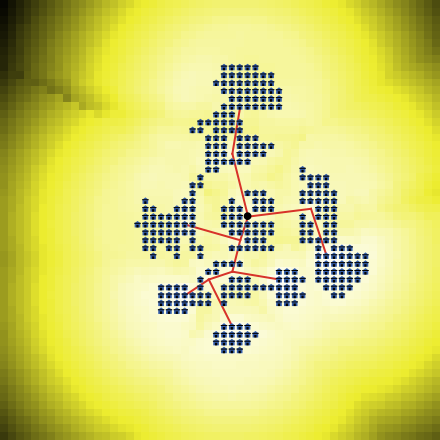
\includegraphics[width=0.65\columnwidth]{figures/lattice}
\caption{\small Exemple de forme urbaine générée par le modèle. La population s’installe autour du réseau (en rouge) relié au centre (en noir). Le contraste des cellules libres est proportionnel à leur valeur, suggérant les étapes suivantes du développement.}
\label{fig_lattice}
\vspace{1cm}
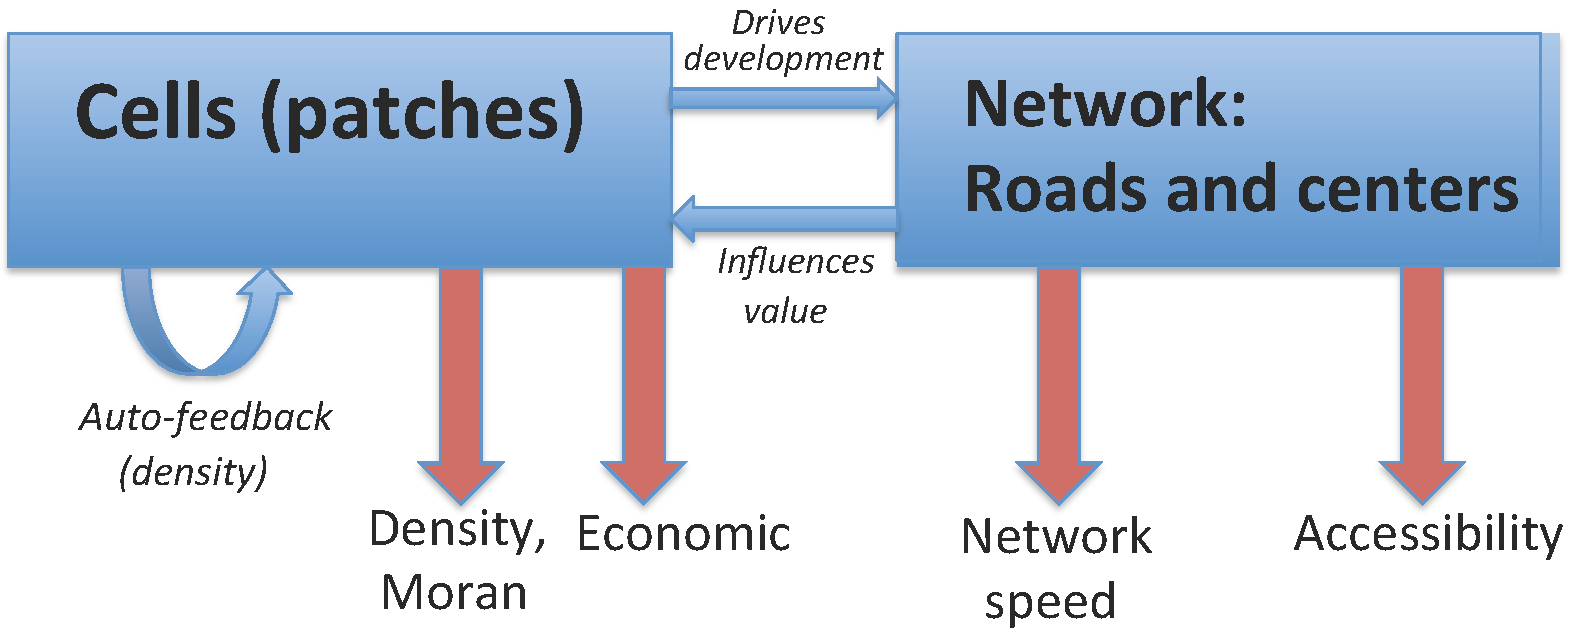
\includegraphics[width=0.8\columnwidth]{figures/flowchart}
\caption{\small Fonctionnement du modèle. \emph{Bleu}: interactions entre agents. \emph{Rouge}: indicateurs d’évaluation.}
\label{fig_flowchart}
\end{figure}

\paragraph{Fonctions d’évaluation}

Lorsque qu’une structure urbaine a été générée, il est nécessaire de pouvoir quantifier ses propriétés par des indicateurs afin par exemple de la comparer à d’autres structures dans un but d’optimisation. Il faut pour cela des indicateurs de performances pour les différents aspects du système pris en compte, qui comprennent la morphologie, la performance du réseau, l’accessibilité fonctionnelle et la performance économique. Les indicateurs peuvent également servir de classifieurs ou discriminants, selon la répartition des valeurs des différentes configurations dans l’espace des indicateurs, c’est à dire qu’un choix pertinent devrait dans ce cas conduire à une classification cohérentes des structures urbaines générées par le modèle. Dans notre cas, les fonctions d’évaluation choisies sont les suivantes.

\begin{itemize}

\item Morphologie : 

La structure morphologique d’une configuration urbaine est définie par la valeur de deux indicateurs $(D,I)$ qui sont la densité intégrée, i.e. la variable $d_1$ intégrée (selon une norme fixée) sur l’ensemble des cellules habitées, et l’indice de Moran de la répartition de la population. L’indice de Moran, représentant l’autocorrelation spatiale de la fonction de densité, est fréquemment utilisé en géographie~\cite{tsai2005quantifying,lenechet:hal-00696445} pour évaluer le caractère polycentrique d’une distribution spatiale de population. Il est défini dans notre cas par 
%
\begin{equation}
I(t)=\frac{M^2}{\sum_{\mu\neq\nu} 1/d_{\mu\nu}}\frac{\sum_{\mu\neq\nu} (P_\mu-\overline{P})(P_\nu-\overline{P})/d_{\mu\nu}}{\sum_{\mu=1}^{M^2}(P_\mu-\overline{P})^2}
\end{equation}
%
où la grille est découpée en $M\times M$ zones carrées d’une échelle intermédiaire entre la taille de la cellule et la taille du monde ($1\ll\!M\ll\!N$), $d_{\mu\nu}$ étant la distance entre les centroïdes des zones $\mu$,$\nu$, les variables $P$ représentant la population totale pour chaque zone ainsi que leur moyenne. Par construction dans $[-1,1]$, des valeurs proches de 1 signifient une distribution monocentrique, 0 une distribution aléatoire et -1 un motif en échiquier (population la plus polycentrique possible).

\item Performance du réseau de transport :

Vu le mécanisme d’extension du réseau par branchements, il ne peut contenir d’autres boucles que celles initialement présentes, rendant des indicateurs comme la robustesse non pertinents. Par contre, comme on modélise un réseau de mobilité, on peut qualifier sa performance de desserte par sa vitesse relative~\cite{banos2012towards}, obtenue par l’intégration de la quantité de détour que le réseau fait par rapport à la ligne droite pour un trajet quelconque.

\item Accessibilité fonctionnelle : 

L’intégration de l’accessibilité aux différentes fonctions sur l’ensemble des cellules, permet après normalisation de définir un indicateur global de performance fonctionnelle de la ville, qui garde un sens sous l’hypothèse que chacun des agents cherche à accéder le mieux possible à chacune des fonctions.


\item Performance économique :

Il est montré dans~\cite{banos2012network} que le modèle de ségrégation de Schelling, un modèle simple de dynamique socio-économique~\cite{schelling1969models}, est extrêmement sensible à la structure spatiale dans lequel il peut être intégré. Cela suggère d’utiliser un modèle similaire afin de mesurer une \emph{performance économique} abstraite d’une configuration urbaine, c’est à dire traduire dans quelle mesure telle structure pourrait influer des dynamiques de ségrégation. Pour cela, on implémente un modèle de dynamique résidentielle inspiré de~\cite{benenson1998multi} permettant de définir un index de ségrégation, par un calcul sur les états stationnaires du modèle obtenus après ajustement des paramètres dans la bonne région du diagramme de phase du modèle de Schelling~\cite{gauvin2009phase}.


\end{itemize}




\subsubsection{Exploration et Analyse de sensibilité}

Le modèle a été implémenté en NetLogo~\cite{NetLogo}, particulièrement adapté pour ce type de modélisation par agents. Les paramètres n’ayant pas de proxys raisonnables sont les poids des variables explicatives $\alpha_k$, pour lesquels une exploration complète de l’hypercube $[0,1]^4$ a été conduite avec un incrément de 0.2 (résultant en un total de $6^4-1=1295$ points, le point $(0,0,0,0)$ étant exclu). Dans le cas d’une configuration initiale aléatoire, des centres urbains (typiquement 4) sont distribués uniformément, et leur activité est tirée uniformément dans $[1,a_{\max}]$. Le réseau initial est construit de façon quasi-déterministe par percolation progressives entre les composantes connexes. Ainsi, une étude statistique du comportement des indicateurs a été conduite afin d’obtenir une validation interne du modèle, ainsi qu’un ordre de grandeur du nombre de répétitions nécessaires pour satisfaire un certain intervalle de confiance sur les indicateurs, qui est fixée à 5 simulations lors de l’exploration de l’espace des paramètres. Concernant l’horizon temporel d’évolution, il est fixé à un maximum dépendant de la taille du monde et correspondant à l’apparition d’effet de bords dans le pire des cas (toujours lorsque  $\alpha_k=(1,0,0,0)$, i.e. lorsque uniquement la densité est prise en compte.


\subsubsection{Résultats}

\paragraph{Formes typiques}

Différentes configuration des paramètres permettent de générer des structures urbaines fondamentalement différentes. En particulier, les formes obtenues pour des points voisins des coins de l’hypercube (une ou deux variable $d_k$ avec poids égaux, les autres de poids nul) fournissent des exemples caractéristiques des types de formes que le modèle peut générer. Le résultat intéressant est qu’on est en mesure de reproduire la ``classification’’ des établissements humains proposée par Le Corbusier en 1945~\cite{mangin2004ville}, suggérant que le modèle peut être admis comme valable à ce degré de simplification (voir Fig.~\ref{fig_corbu}).



\begin{figure}
\centering
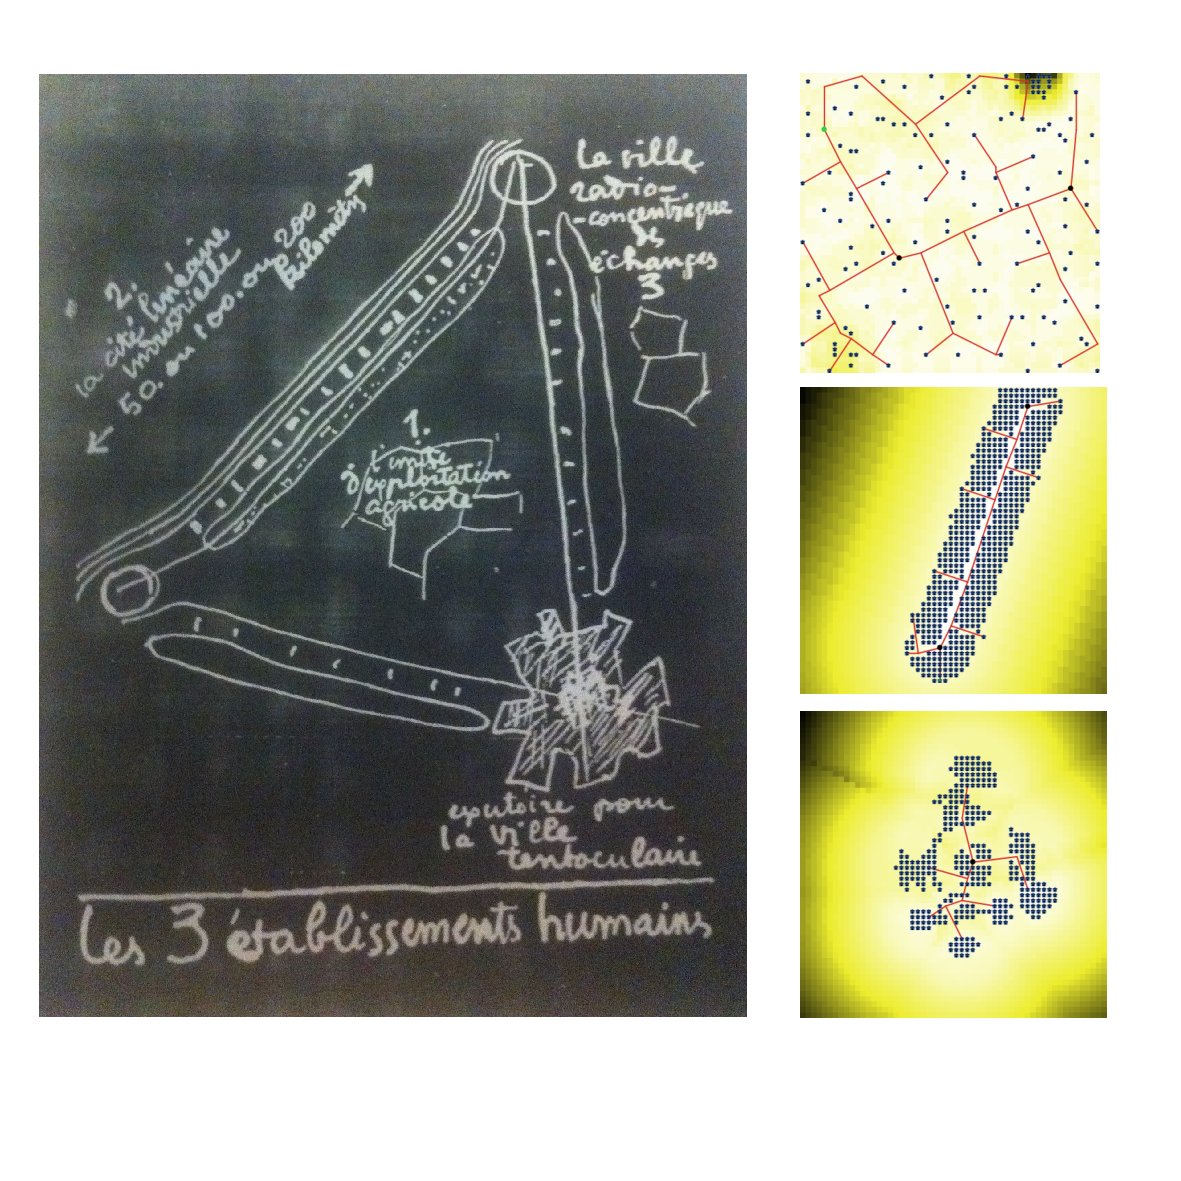
\includegraphics[trim=0mm 18mm 2mm 12mm, clip, width=\columnwidth]{figures/corbu}
\caption{\small Formes typiques obtenues par le modèle, reproduisant les trois types d’établissement proposés par Le Corbusier que sont les villes radio-concentriques, les cités linéaires et les communautés rurales. La typologie est reproduite avec les poids suivants : \emph{Haut}: $(\alpha_k)=(1,0,0,0)$, i.e.~densité uniquement. \emph{Millieu}: $(0,1,0,0)$, i.e.~distance aux routes. \emph{Bas}: $(0.2,0,1,0)$, i.e.~réseau et densité. \emph{Gauche}: source~\cite{mangin2004ville}.}
\label{fig_corbu}
\end{figure}

\begin{figure}
\centering
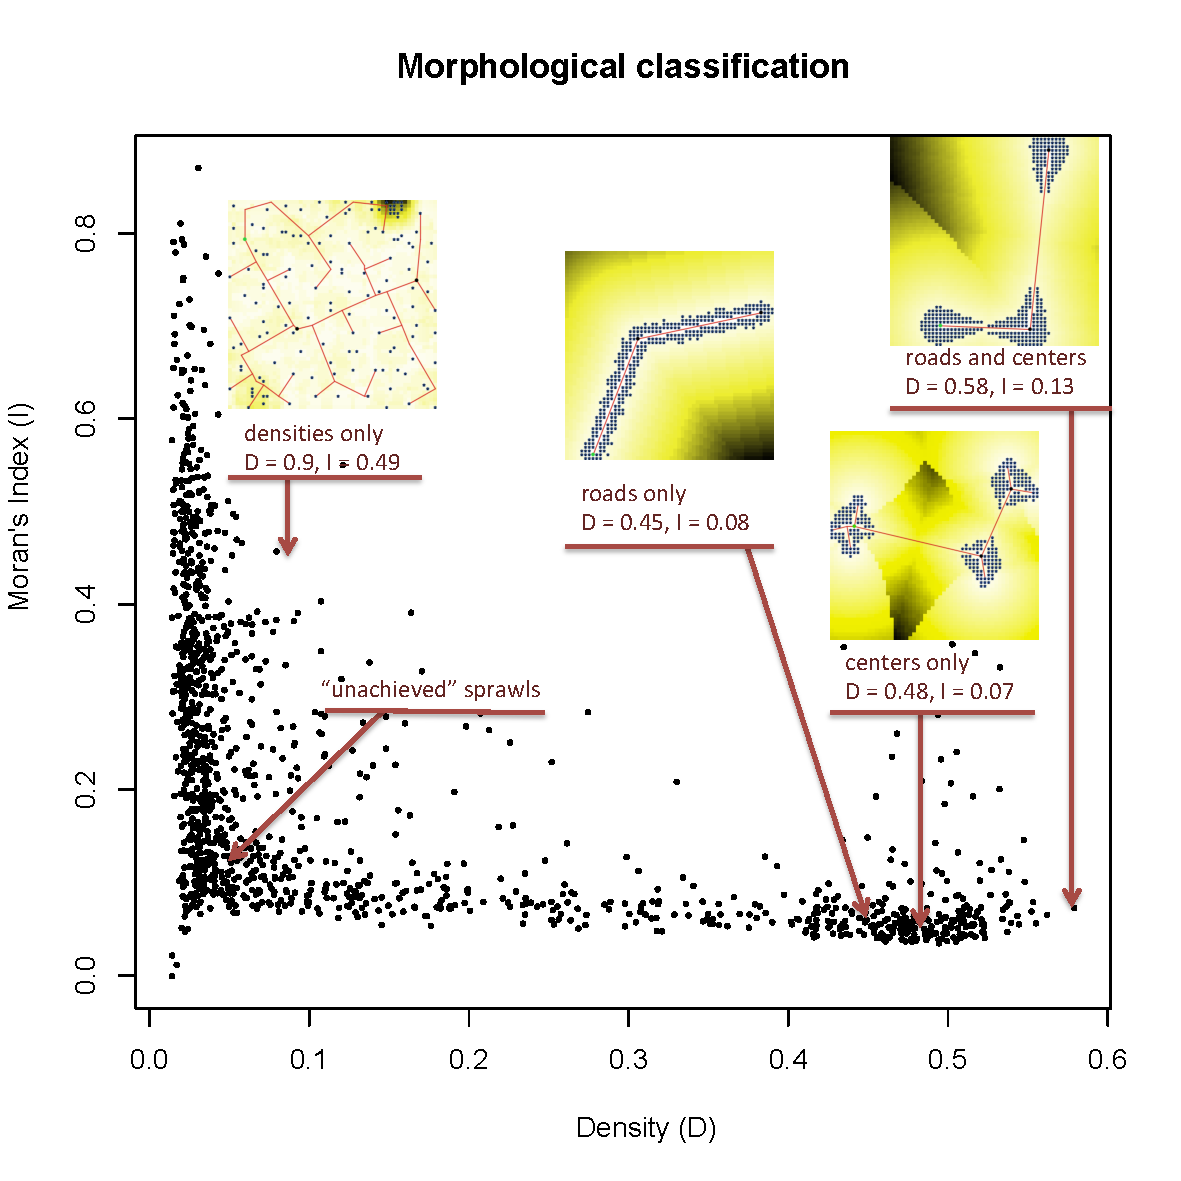
\includegraphics[trim=0mm 5mm 0mm 23mm, clip, width=\columnwidth]{figures/morpho}
\caption{\small Classification morphologique des formes urbaines.}
\label{fig_morpho}
\end{figure}

\paragraph{Classification des structures}

A partir des indicateurs morphologiques définis ci-dessus, on est en mesure d’extraire une classification des structures, correspondant à différentes ``classes’’ dans le plan $(D,I)$. C’est un résultat intéressant dans le sens où cela permet de mieux cerner l’influence de chaque paramètre sur la forme urbain finale.

\paragraph{Application à un cas concret : optimisation d’un configuration urbaine}

Les autres indicateurs jouent un rôle dans l’application du modèle à un cas concret, que nous ne présentons pas ici. Globalement, on est en mesure de représenter une politique urbaine par la répartition des centres initiaux et de leur activités, et donc de comparer les performances des différentes politiques par les sorties du modèle appliqué à cette configuration initiale.

\subsubsection{Conclusion}

Cette étude de cas montre ainsi qu’un couplage complexe entre évolution de la ville et du réseau est possible à ce degré d’élaboration, ce qui est encourageant pour la recherche de modèles plus raffinés dans notre thèse. De nombreuses extension sont par exemple possible à ce modèle, comme des règles d’évolution du réseau additionnelles, ou des règles de valeur des cellules vérifiant des modèles microéconomiques.








%% II - Transportation Network Morphogenesis

\subsection{Morphogenèse d'un réseau de transports}


\subsubsection{Présentation}

La question de l’établissement de règles pour la croissance d’un réseau, qui sera essentielle à notre problème, a connu récemment de nombreux développements notamment grâce à l’influence de l’étude de systèmes complexes biologiques. A l’instar des techniques d’ingénierie morphogénétique qui consistent à concevoir des systèmes artificiels cherchant à reproduire les propriétés d’auto-organisation de systèmes vivants \cite{doursat2012morphogenetic}, des analogies entre des propriétés d’établissement de réseau optimal d’un certain type de moisissure et les propriétés de réseaux de transports ont été proposées afin de comprendre d’une part la forme des réseaux actuels et de pouvoir aider à des décisions de planification d’autre part~\cite{adamatzky2010road,Bebber22092007}. Nous inspirant d’un modèle simple de croissance de réseau de ce type proposé dans~\cite{TeroAl10}, nous étudions les possibilités de morphogenèse de réseau de cette façon. L’objectif est de pouvoir créer un réseau cohérent à partir d’un espace initial homogène, en répondant à des demandes successives de transport.


\subsubsection{Description du modèle}

Considérant un espace homogène et isotrope, dans lequel les déplacements peuvent s'assimiler à des flux, on le discrétise en une grille. Les sommets sont reliés par des arêtes représentant les tubes dans lequel un fluide peut circuler. Ainsi, chaque sommet est caractérisé par sa pression $p_{i}$. Le tube $ij$ a un diamètre $D_{ij}$, une longueur $L_{ij}$ et est traversé par un flux $Q_{ij}$. L'équation d'évolution des diamètres des tubes en fonction du flux les parcourant est typiquement de la forme suivante : avec $D_{ij}$diamètre du tube $ij$ ,$Q_{ij}$ flux à travers le tube $ij$ et $\gamma=1,8$ paramètre fixé,

\begin{equation}
\frac{dD_{ij}}{dt}=\frac{\left|Q_{ij}\right|^{\gamma}}{1+\left|Q_{ij}\right|^{\gamma}}-D_{ij}
\end{equation}

D'autre part, on a l'équivalent de la loi d'Ohm pour les pressions du fluide

\begin{equation}
Q_{ij}=\frac{D_{ij}}{L_{ij}}\cdot(p_{i}-p_{j})=K_{ij}\cdot(p_{i}-p_{j})
\end{equation}

en posant $K_{ij}=\frac{D_{ij}}{L_{ij}}$.

On obtient, en écrivant la conservation des flux pour chaque noeud, et en combinant les équations, un système linéaire à résoudre afin de trouver l'ensemble des pressions dans le réseau à un instant donné, étant donné des flux constants (de somme nulle) correspondant au fluide entrant et sortant du système. Le système est inversible, ce qui permet une implémentation rapide d'une itération des diamètres des tubes. Il est intéressant de remarquer que le système est analogue à un système électrique, les pressions correspondant aux tensions, et les $K_{ij}$ aux impédances des arêtes (les lois de Kirschoff étant analogues aux équations ci-dessus).

\subsubsection{Résultats}

\paragraph{Génération d’un réseau}

Etant donné une configuration initiale de pôles à desservir, qui correspondent aux points parmi lesquels une origine et une destination sont tirés à chaque itération, et qui sont dans ce cas respectivement source et puits des flux circulant dans le réseau, on peut itérer le modèle à partir d’une grille uniforme. On obtient au bout d’un certain nombre d’itérations convergence de la forme du réseau subsistant, qu’on peut alors extraire. La figure~\ref{fig:exNW} montre un exemple des réseaux qu’on peut obtenir.


\begin{figure}
\centering
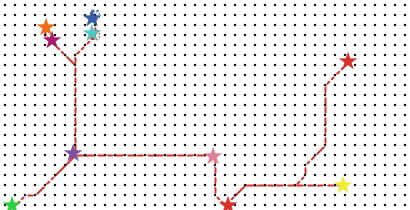
\includegraphics[width=\textwidth]{/Users/Juste/Documents/ComplexSystems/ProjetNetworkGeneration/Docs/networkLessDense}\\[20pt]
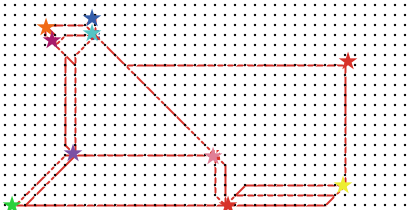
\includegraphics[width=\textwidth]{/Users/Juste/Documents/ComplexSystems/ProjetNetworkGeneration/Docs/networkDense}
\caption{\small Exemple de réseaux obtenus par itérations successives du modèle sur une grille initiale uniforme. Les étoiles correspondent aux différents pôles à desservir. En haut, les paramètres conduisent à un réseau sans boucles ($\gamma$ grand) tandis que d’autres valeurs donnent des réseaux redondants plus robustes (en bas).}
\label{fig:exNW}
\end{figure}


\paragraph{Application à des données géographiques}

Le modèle peut facilement être intégré dans un Système d’information géographique (dans notre cas via l’extension GIS de Netlogo). On peut ainsi contraindre l’évolution du réseau à une topographie de routes existantes, dans le but par exemple de déterminer un itinéraire optimal pour une nouvelle ligne de transport en commun. Il est surtout intéressant d’observer l’émergence du réseau final au sein d’un environnement contraint, et constater que les règles utilisées fonctionnent toujours dans ce cadre. Voir fig.~\ref{fig:applicationGIS} pour un résultat de l’application à un cas concret sur des données géographiques.

\begin{figure}
\centering
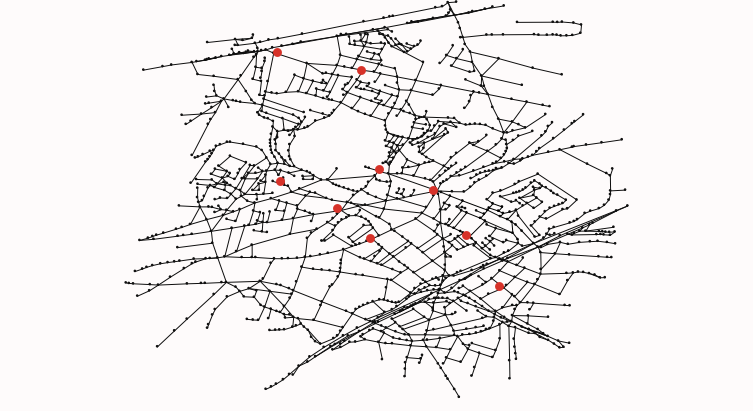
\includegraphics[width=0.45\textwidth]{/Users/Juste/Documents/ComplexSystems/ProjetNetworkGeneration/NetworkGeneration/Results/Romainville/tick1}
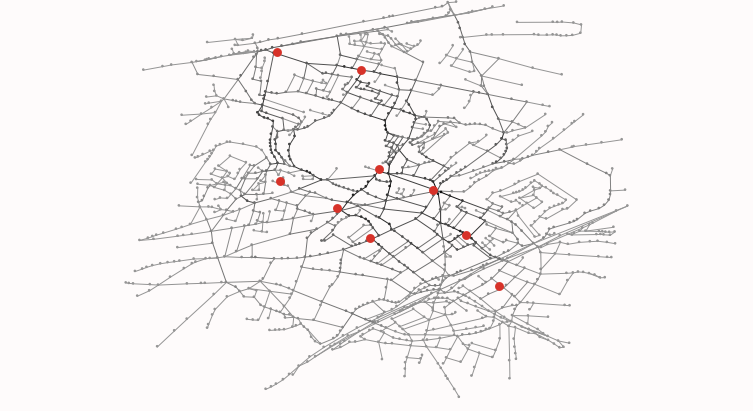
\includegraphics[width=0.45\textwidth]{/Users/Juste/Documents/ComplexSystems/ProjetNetworkGeneration/NetworkGeneration/Results/Romainville/tick20}\\
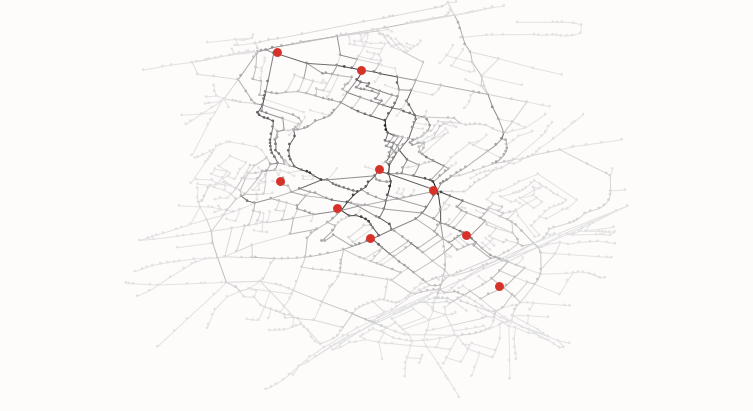
\includegraphics[width=0.45\textwidth]{/Users/Juste/Documents/ComplexSystems/ProjetNetworkGeneration/NetworkGeneration/Results/Romainville/tick50}
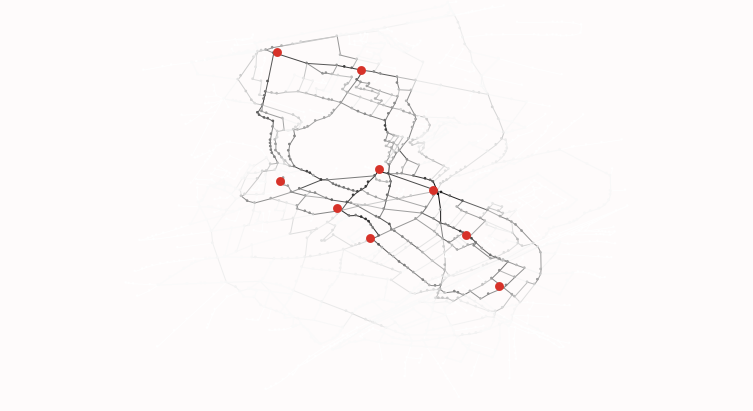
\includegraphics[width=0.45\textwidth]{/Users/Juste/Documents/ComplexSystems/ProjetNetworkGeneration/NetworkGeneration/Results/Romainville/tick101}
\caption{\small Application à des données géographiques. De haut en bas et de gauche à droite, l’état du réseau à différents pas de temps (1, 10, 50 et 100), les pôles à desservir en rouge. On observe bien l’émergence  progressive d’un réseau qui vérifie certains critères d’optimalité (robustesse et coût à robustesse fixée).}
\label{fig:applicationGIS}
\end{figure}



\subsubsection{Conclusion}

Ce second exemple nous montre un cas de réseau auto-généré par des règles relativement simples, qui permettent d’obtenir toutefois des réseaux relativement élaborés. Dans notre cadre, il est intéressant de voir que des modèles simples sont rapidement accessibles, et dans ce cas peuvent facilement être couplés avec une dynamique urbaine (pôles de desserte).





\newpage


\section*{Conclusion}

Le projet présenté nous a conduit à des développements méthodologiques faisant partie intégrante de celui-ci, car il est nécessaire de fixer un certain nombre de points au préalable pour éviter de s’égarer dans un sujet potentiellement bien plus vaste qu’une seule thèse. On a également renforcé le projet par deux études de cas montrant une première approche dans les deux domaines au coeur du sujet que sont la modélisation de la croissance urbaine et la modélisation de la croissance des réseaux, et dont le couplage semble entrer dans un domaine de faisabilité raisonnable.

\vspace{1cm}

Ainsi, on essayera au cours de cette thèse d'approfondir les connaissances sur les interactions réciproques entre transports et urbanisme en liant les approches de modélisation de l'évolution de la ville à celles de modélisation de croissance des réseaux, tout en gardant l'objectif d'obtenir des modèles opérationnels pouvant guider l'aide à la décision. On répondra donc à deux enjeux essentiels, l'un d'application directe concernant la planification des infrastructures de transport, en se plaçant dans le cadre plus global de l'autre qui est la contribution à l'un des volets clés de la Feuille de Route actuelle pour les Systèmes Complexes~\footnote{http://roadmaps.csregistry.org/tiki-index.php?page=French+Roadmap} qui est la compréhension des systèmes urbains et territoriaux.

\newpage{}

\bibliographystyle{apalike-fr}
\bibliography{/Users/Juste/Documents/ComplexSystems/Misc/ProjetThese/Biblio/these,/Users/Juste/Documents/ComplexSystems/Biblio/BibTeX/global,/Users/Juste/Documents/ComplexSystems/CCUPD/Biblio/ccupd,/Users/Juste/Documents/Cours/ComplexSystemsMadeSimple/UrbanMorphogenesis/Biblio/projetCSMS,/Users/Juste/Documents/ComplexSystems/ProjetNetworkGeneration/NetworkGeneration/Biblio/NWGeneration}












\end{document}



